\subsection{Applying linear regression to the data set}
All the parameters have been normalized, before doing the sequential feature selection and linear regression. A 10-fold cross validation with a 10-fold internal cross validation method have been used for selecting the features for the model. The figure below (figure \ref{fig:selected_features}.) shows the selected features at each fold. 

\vspace{-5pt}
%kommentar
\begin{figure}[!ht]
	\centering
	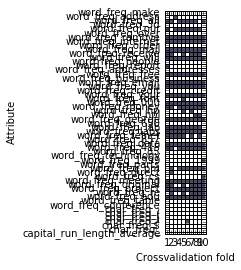
\includegraphics[width=0.7\textwidth]{Fig/regression_1.png}
	\vspace{-5pt}
	\caption{Selected features}
	\label{fig:selected_features}
\end{figure}

By doing feature selection we reduce the amount of data, by only selecting the attributes which correlates to out regression problem. This makes modelling the data less prone to over fitting and reduces the overall complexity of the model. However when comparing the regression errors with feature selection and with out feature selection, the difference seems almost indistinguishable see table (figure \ref{tab:feature_selection_vs_no}.), thus the model with feature selection is far less complex as described.

\begin{table}[!ht]
  	\centering
  		\begin{tabular}{ccc}
  			\hline
  			 Measure & Without feature selection & With feature selection\\ \hline \hline
  			Test error & 0.938505700248 & 0.940197192727 \\
  			Training error & 0.923006656194 & 0.928276304747 \\ \hline
  		\end{tabular}
	\caption{Error difference between with and without feature selection}
  	\label{tab:feature_selection_vs_no}
\end{table}

The figure below (figure 2) shows the regression for the first fold and for the 10th fold. Here it illustrates how the squared error gets lower and lower for each training session we do with the model. 

\vspace{-5pt}
\begin{figure}[!ht]
\centering

\begin{subfigure}[b]{.45\linewidth}
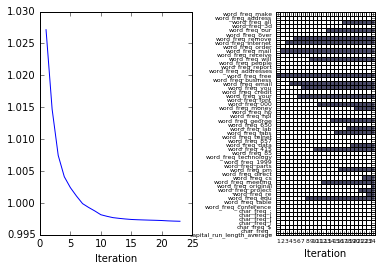
\includegraphics[width=\linewidth]{Fig/regression_first_fold.png}
\caption{First fold}
\end{subfigure}
\begin{subfigure}[b]{.45\linewidth}
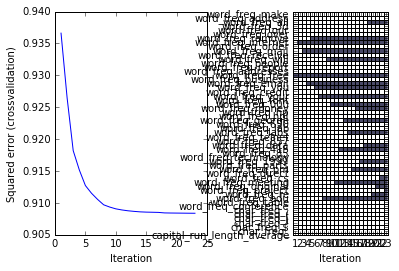
\includegraphics[width=\linewidth]{Fig/regression_10th_fold.png}
\caption{10th fold}
\end{subfigure}

\label{fig:first_vs_10th}
\caption{First fold compared with 10th fold of the linear regression}
\end{figure}
  